\section{Data}
The main input of the Articles/Editors ranking method is the binary matrix $\mathbf{M_{e,a}}$ which determines, for a category on Wikipedia, which articles have been modified at least once by each editor. We collected all contribution data for all articles in 10 categories (c.f. table \ref{tab:statistics} for summary statistics on the categories). In addition, we made 10 snapshots of equal number of edits to account for the evolution over time of each category (see Figure \ref{fig:accumulative_snapshots}). For each snapshot, $\mathbf{M_{e,a}} =1$ if editor $e$ has modified article $a$ up to the snapshot, $\mathbf{M_{e,a}} =0$ otherwise. The final snapshot represents the entire history of the category up to the date of data collection (i.e., February 14, 2014).

\begin{tabular}{llll}
\toprule
Category & Users & Articles &  Edits \\
\midrule
2013 films &  5215 &     1896 &  150956 \\
American male novelists &  9946 &     2460 &  224783 \\
American women novelists &  5968 &     1936 &  138716 \\
Bicycle parts &   210 &       70 &    4981 \\
Computability theory &   272 &       92 &    7117 \\
Counterculture festivals &   578 &       66 &   10515 \\
Economic theories &  1145 &      212 &   28658 \\
Feminist writers &  1357 &      233 &   25738 \\
Military history of the US &   854 &      180 &   20172 \\
Nobel Peace Prize laureates &  4165 &      104 &   91522 \\
Sexual acts &  2190 &       93 &   45901 \\
Yoga &   730 &      123 &   25315 \\
\bottomrule
\label{tab:statistics}
\end{tabular}

\begin{figure}[!t]
\centering
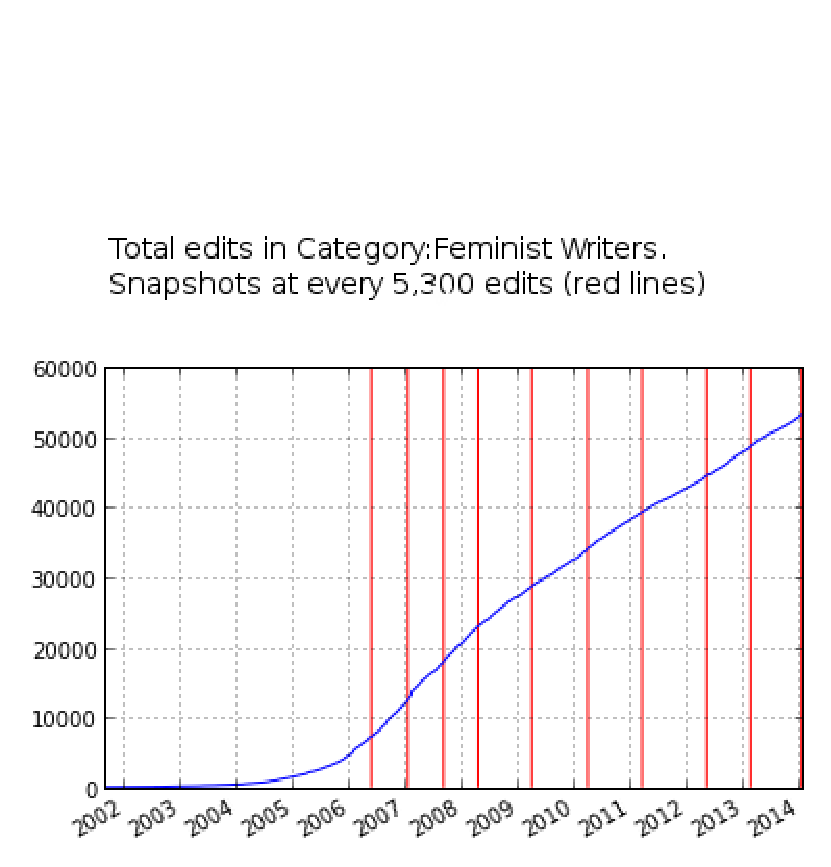
\includegraphics[width=0.9\columnwidth]{Figures/cumulative_snapshots_Feminist_Writers.eps}
\caption{Typical snapshots for a category of Wikipedia (here, \textit{\textbf{Feminist Writers}} with one snapshot every 5,300 edits). As contributions go on, snapshots incorporate more information on whose editors have modified the articles in a category, hence filling further the matrix $\mathbf{M}$ (see Figure \ref{fig:matrix}).}
\label{fig:figure1}
\end{figure}

To calibrate the editors/articles ranking method, namely $\alpha$ and $\beta$, we also collected expertise data for editors and quality metrics for articles, which are unrelated to the number of edits, and are considered as state-of-the-art metric although there is no consensus on expertise (resp. quality) of editors (resp. articles) on Wikipedia. The exogenous metric for editors $v_e$ we take is {\it labour hours} as defined by  \cite{halfaker/geiger}. The labor hours metric is determined by the number of hours between the first and the last edit of session of edits, in which two consecutive edits occur no longer than 1 hour from each others {\bf [Max, please confirm that I understood rightly, and also provide the reference ? ]}. {\bf [By the way, can you say in a nutshell why this metric is great ? or at least better than any other ?]}. There is no one single quality metric for articles. We therefore use a combination of five metrics : (i) ratio of mark-up to readable text, (ii) number of headings, (iii) article length, (iv) citations per article length, and (v) outgoing intrawiki links \cite{wang2013tell,klein2014investigating}. We performed a Principal Component Analysis (PCA) , and reduced the five dimensions to the direction (first eigenvector) of
 maximum variance. This aggregate metric $v_a$ accounts for between 50\% and 70\% of the variance, and thus recalls well the quality of articles. Both metrics are calculated for each category and each snapshot. For our model calibration purpose, $v_e$ and $v_a$ are the state-of-the-art and assumed to be the {\it Grand Truth}, even though their ability to reflect well expertise and quality remains questionable (see Section \ref{limitations} for further discussion).
